

Diese Projektgruppe des ELISE Projektes wird dem Lehrstuhl Medizinische Informatik \& Mikrosystementwurf und dem Lehrstuhl f{\"u}r Mustererkennung zugeordnet. \\

Die Gruppe wird von Dr.-Ing. Armin Gr{\"u}newald, David Kr{\"o}nert und Frédéric Li geleitet. 
Innerhalb der Gruppe wurden dazu unabh{\"a}ndig ein Sprecher und ein stellvertretender Sprecher von den Gruppenmitgliedern gew{\"a}hlt. Als Projektgruppensprecher wurde Artur Piet und als Stellvertreter Jonas P{\"o}hler ausgew{\"a}hlt. 
Diese Stellung ist jedoch nicht die eines Leiters mit Entscheidungs- und Weisungsbefugnissen. Die Sprecher sind also auf die Kooperationsbereitschaft der anderen Gruppenmitglieder angewiesen. 
Konkrete Aufgaben der Sprecher waren unter anderen das Verteilen von Verantwortungsbereichen auf alle Mitglieder, die Einf{\"u}hrung von regelm{\"a}{\ss}igen Gruppentreffen um den {\"u}berblick {\"u}ber alle Fortschritte zu garantieren und die {\"u}bernahme m{\"o}glichst aller organisatorischer T{\"a}tigkeiten (z.B. Messreihen organisieren, Beschaffungsprozesse koordinieren, usw.). \\

Die Laufzeit der Projektgruppe wurde auf etwa 1 Jahr gesetzt, wobei das Kick-Off Meeting am 23.10.2017 stattfand. Der geforderte individuelle Zeitaufwand aller Gruppenmitglieder entspricht der jeweils im Modulhandbuch des Studienganges definierten Leistungspunkte f{\"u}r die Projektarbeit, also 600 Stunden f{\"u}r Jonas P{\"o}hler, Arnaud Eric Toham Waffo, Boris Kamdem, Kevin Orth, Meryem Dural sowie Minas Michail und 270 Stunden f{\"u}r Artur Piet. Es folgt ein Balkendiagramm mit den geforderten Stunden im Verlgeich zum tats{\"a}lichem Zeitaufwand. \\

\begin{figure}[h]
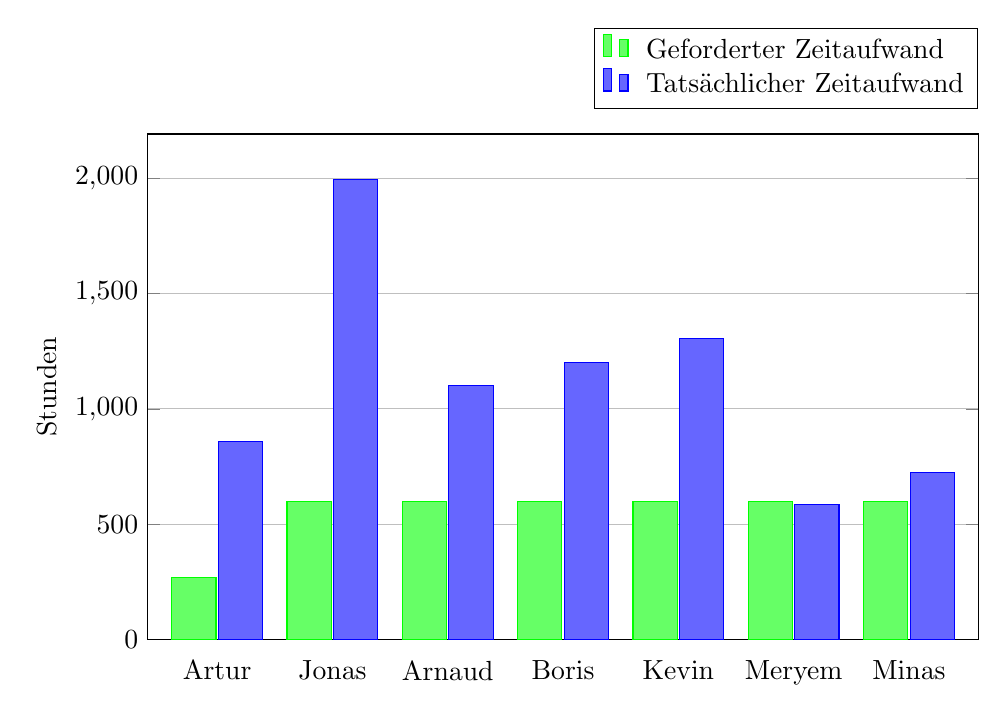
\begin{tikzpicture}
    \begin{axis}[
        width  = \textwidth,
        height = 8cm,
        major x tick style = transparent,
        ybar=2*\pgflinewidth,
        bar width=16pt,
        ymajorgrids = true,
        ylabel = {Stunden},
        symbolic x coords={Artur,Jonas,Arnaud,Boris,Kevin,Meryem,Minas},
        xtick = data,
        scaled y ticks = false,
        enlarge x limits=0.1,
        ymin=0,
        legend cell align=left,
        legend style={
                at={(1,1.05)},
                anchor=south east,
                column sep=1ex
        }
    ]
        \addplot[style={green,fill=green!60,mark=none}]
            coordinates {(Artur, 270) (Jonas,600) (Arnaud,600) (Boris,600) (Kevin,600) (Meryem,600) (Minas,600)};

        \addplot[style={blue,fill=blue!60,mark=none}]
             coordinates {(Artur,857) (Jonas,1993) (Arnaud,1100) (Boris,1200) (Kevin,1304) (Meryem,587) (Minas,722)};


        \legend{Geforderter Zeitaufwand,Tats{\"a}chlicher Zeitaufwand}
    \end{axis}
\end{tikzpicture} 
%\caption{Stundenaufwand: Vergleich zwischen gefoderten und tats{\"a}chlichen Zeitaufwand der Projektgruppenmitglieder.} 
\end{figure} 



\subsection{Verantwortungsbereiche}


Innerhalb der Projektgruppe (PG) war ein Ziel, dass jeder der Mitglieder "Experte" f{\"u}r einen Bereich wird. Damit haben wir die Verantwortung relativ gleichm{\"a}{\ss}ig auf alle aufgeteilt. Dazu muss noch erw{\"a}hnt werden, dass die Teammitglieder nicht nur ausschlie{\ss}lich die Aufgaben des jeweiligen Verantwortungsbereiches erlegibt habe. Es wurde sich vielmehr gegenseitig immer unterst{\"u}tzt und viel zusammengearbeitet. Die Verantwortungsbereiche haben sich mit der Zeit folgenderma{\ss}en aufgeteilt:

\begin{itemize} \setlength\itemsep{-0.15cm}
  \item Artur Piet: Mustererkennung, 3D-Konstruktion, Berichtserstellung und Sprecher der PG
  \item Jonas P{\"o}hler: Hardware, Webanbindung, VR Szenarien und Stellv. Sprecher der PG
  \item Arnaud Eric Toham Waffo: Plan B
  \item Boris Kamdem: Langeweile-Szenario sowie Fragebogen in VR und Plan B
  \item Kevin Orth: Komplette Hardware
  \item Meryem Dural: Frustations-Szenario in VR und Plan B
  \item Minas Michail: WarmUp- und Gl{\"u}cks-Szenario, Zusammenführung / Verknüpfung der VR-Szenarien in einer Unreal-Datei, Plan B
\end{itemize}




\subsection{Gruppentreffen}


Die w{\"o}chentliche Gruppentreffen finden immer Donnerstags ab 14:00 Uhr statt und beginnen in der Regel mit einer Update-Runde. Hierbei kommen alle Gruppenteilnehmer der Reihe nach dran und jeder erkl{\"a}rt kurz woran letzte Woche gearbeitet wurde, was die aktuellen Herausfoderungen und Probleme sind und was genau als n{\"a}chstes geplant ist. Ziel ist es den Austausch und die Kommunikation unter den Teammitgliedern und den Projektleitern zu f{\"o}rdern, damit alle Teilnehmer auf dem selben Wissenstand sind, da einzelnen Aufgaben durchaus gro{\ss}en Einflu{\ss} auf T{\"a}tigkeiten von anderen Mitgliedern haben k{\"o}nnen. \\